% 這份檔案由 make_latex.py 產生，不要直接手改；請改 paper.typ。
% 中文排版用 ctexart + xelatex（見 build_tex.bat）。
\documentclass[11pt,a4paper]{ctexart}
\usepackage[margin=2.4cm]{geometry}
\usepackage{amsmath,amssymb}
\usepackage{calc}
\usepackage{graphicx}
\usepackage{booktabs}
\usepackage{longtable}
\usepackage{array}
\usepackage[numbers]{natbib}
\usepackage{hyperref}
% CJK 段落常因缺少斷行點而溢出邊界；放寬斷行伸縮量（只影響間距，不影響內容）。
\emergencystretch=3em

\title{量子分類器的容量斷崖與校準消融\\[0.35em]\large Capacity Cliff and Calibration Ablation in a Hybrid Quantum--Classical Classifier}
\author{Xin Yang、Poyuan Chung、Yuan-Liang Zhong\\\parbox{0.86\textwidth}{\centering 中原大學物理系（Department of Physics, Chung Yuan Christian University），台灣桃園}}
\date{}

\begin{document}
\maketitle

\begin{abstract}
\textbf{摘要}------本研究的目標是「用量子電路當分類器輸出層」這條路線的\textbf{受控檢驗}，
而非追求量子優勢。我們以 Wang
等人（2026）的混合式貝氏量子---古典分類器為基準， 用 CUDA-Q 複現其 4
qubit 量子層，並延伸兩項該研究未涵蓋的實驗：
（一）\textbf{容量斷崖}：掃描 qubit 數與電路深度，檢驗效能是否單調；
（二）\textbf{校準消融}：施加去相位算子使量子層古典化，量測其對校準品質的邊際貢獻。
所有量子電路結果都以 CUDA-Q（正式軌）與一個獨立實作的純 NumPy
狀態向量模擬器 （練習軌）各算一次並比對機率向量：複現管線一致到
\(4.16 \times 10^{- 17}\)， 容量掃描的最大電路（250 閘）一致到
\(3.47 \times 10^{- 18}\)，消融電路一致到 \(8.33 \times 10^{- 17}\)。
我們明確不主張任何量子優勢：5 個 qubit 的狀態向量僅 512
位元組，完全可被古典模擬。
本研究的貢獻在於提供一條\textbf{可完全驗證}的管線與\textbf{可證偽}的實驗設計。

\textbf{關鍵詞}------量子貝葉斯網路、混合式量子---古典學習、校準、不確定性量化、CUDA-Q
\end{abstract}
\section{引言}

深度學習分類器的最後一層通常輸出 \textbf{softmax}
分布------把一組實數取指數後歸一化， 使其總和為
\(1\)，因此形式上像是一組機率。但這組數字\textbf{不是}校準過的機率：
它經常系統性過度自信 \cite{guo2017}。
所謂\textbf{校準}（calibration），指的是「模型自己宣稱的信心」與「它實際答對的頻率」
是否相符------一個宣稱 \(90\%\) 信心卻只答對 \(70\%\)
的模型，即使準確率很高也不可信。在需要可信信心的場域（醫療、金融、教育），這個問題不能只靠準確率來評估。

近年出現一類混合式架構：以古典網路抽取特徵，再以量子電路作為決策層
\cite{wang2026}。這類工作報告了準確率與校準的改善，但有一個共同的結構性特徵------
\textbf{量子層在消融實驗中從未被當成受控變因}。 以 \cite{wang2026}
為例，其最先進的設計是「唯一變因」比較：
所有模型共享相同前處理與分類頭，只改第一層卷積為貝氏或確定性。
量子層在兩組對照中是完全相同的常數。

因此該研究------以及同類工作------\textbf{無法回答「量子性本身是否必要」}。
本研究補上這一步。

\textbf{貢獻摘要}

\begin{enumerate}
\item
  提出\textbf{去相位消融}：以 Tucci 的古典化算子 \cite{tucci2012}
  作為\textbf{同一模型內}的唯一變因，
  （不換模型、不換資料、不換參數量）檢驗量子性對校準與容量的邊際貢獻。
  在我們檢索的範圍內未發現既有工作以此為消融工具------最接近者或是以糾纏度作觀測性歸因
  \cite{nausheen2026}，或是以退極化雜訊作外部變因 \cite{ghosh2026}。
\item
  把\textbf{容量斷崖}掃描延伸到 qubit 數 \(3\)--\(10\) \(\times\)
  電路深度 \(1\)--\(8\)。既有工作已建立 \((Q,L)\) 的縮放 協定並報告飽和
  \cite{vyskubov2026}，亦已在單一軸上觀察到非單調（\cite{le2025} 的 qubit
  軸； \cite{zhang2021suppression}
  的深度軸）。我們補上的是\textbf{固定讀出規則}下的完整二維網格、\textbf{同時報告校準}，
  以及一項既有工作未報告的現象：\textbf{測試準確率隨 qubit
  數下降}------在容量真正被用上的配置上成立 （各 \(n\)
  的峰值與最深切面自 \(n = 4\) 起單調），較淺的切面則被最佳化不足掩蓋。
  （\(n \geq 3\) 是硬需求：8 個類別機率最少需要 3 個 qubit
  的投影讀出。）
\item
  以 CUDA-Q 複現 \cite{wang2026} 的 4 qubit 量子層，並與獨立 NumPy
  實作交叉驗證（\(4.16 \times 10^{- 17}\)）；
  此項定位為\textbf{可重現性證據}，而非方法論貢獻。第 6
  節的兩項實驗另經正式軌背書： 容量掃描的最大電路
  \(3.47 \times 10^{- 18}\)、消融電路 \(8.33 \times 10^{- 17}\)。
\item
  誠實報告三個否定性結論（見第 6 節）。
\end{enumerate}

\section{相關工作}

\subsection{混合式量子---古典分類器}

\cite{wang2026} 的三階段骨架為「古典特徵抽取 → 量子態演化 → 古典決策」，
量子層使用 4 個量子位元（qubit）、電路深度 2 的參數化量子電路
（parameterised quantum circuit, PQC）， 讀出方式為量測全部 qubit 的
Pauli-\(Z\) 期望值成一個向量，再交由線性層分類。
其增益明確來自\textbf{古典貝氏前端}：MNIST（手寫數字影像資料集）\(+ 2.32\)
個百分點、 Fashion-MNIST（服飾影像資料集）\(+ 5.61\) 個百分點，
而量子層固定不變。

\subsection{容量與蒸餾的已知限制}

\cite{wada2025} 在靜態詞嵌入的蒸餾研究中報告了兩個相關現象：
其一，學生維度降至 \(d = 64\)
時，知識蒸餾反而使效能劣化（\(63.8 \rightarrow 52.5\)）；
其二，改用更強的老師（GTE-large，一種通用文字嵌入模型）反而使學生變差
（\(62.9\) 對比 GTE-base 的 \(63.8\)）， 作者歸因於師生容量差距過大。
本研究檢驗同一類「容量差距過大即失效」的現象是否出現在量子決策層。

\subsection{量子貝葉斯網路}

\cite{tucci2012} 將古典貝氏網路的節點由條件機率表推廣為量子通道，
並指出對節點施加去相位算子 \(\operatorname{cl}\)
會使整個網路退化為古典貝氏網路。
這個算子構成本研究消融實驗的理論基礎：它是一個\textbf{精確的古典化映射}，
因此「量子 vs 古典」不需要更換模型、資料或參數量。

\subsection{把量子性當成受控變因}

與本研究最接近的三件工作各走了一條不同的路，也都留下了本研究要補的缺口。

\cite{jafari2026} 以\textbf{複數值么正表徵}取代 softmax
作為分類頭：共用同一個骨幹、只換輕量分類頭。 在 CIFAR-10（10
類彩色影像資料集）上它把期望校準誤差 （expected calibration error,
ECE）從 \(0.0355\) 降到 \(0.0146\)， 但同一組實驗中把讀出換成 Born
律（以波函數振幅的平方作為機率）反而\textbf{惡化}到 \(0.0819\)。
這有兩層意義：一是這種「唯一變因」式的消融確實可行；二是\textbf{量子式的讀出本身不是校準的保證}。
不過該研究的變因是\textbf{表徵形式}（複數么正對實數），且其么正層由
Cayley 映射（把反 Hermitian 矩陣映到么正矩陣的一種參數化）參數化、
可在古典硬體上精確執行，因此它隔離的仍然不是「量子性」。

\cite{nausheen2026} 在釋義偵測（paraphrase
detection，判斷兩句話是否同義）任務上， 以 Meyer--Wallach
糾纏度（一種多體糾纏程度的量度）對效能作\textbf{觀測性}歸因（\(r = 0.85\)）。但相關不是介入：糾纏度與電路深度、參數量同步變動，無法排除混淆。

\cite{ghosh2026} 改以\textbf{退極化雜訊}作外部變因，掃描變分分類器的
ECE， 發現 ECE 不隨雜訊單調上升，並警告表達力較差的 ansatz
可能只因塌縮到退化解而看似校準良好。

三者的共同缺口是：量子性本身從未成為\textbf{同一模型內}的唯一變因。
本研究以 \cite{tucci2012} 的古典化算子填補這個位置，並採納
\cite{ghosh2026} 的警告， 對每個（臂, 種子）另外記錄塌縮指標。

\section{理論基礎}

本節把「去相位消融為什麼有效、以及在什麼位置才有效」寫成可證明的命題，
並且\textbf{只使用指定的兩本大學用書}------Griffiths 與
Schroeter（以下記為 \textbf{G}） 以及 Arfken、Weber 與
Harris（\textbf{A}）------所涵蓋的工具。
需要的背景只有大學量子力學：密度算符、投影算符、么正變換與交換子。

\begin{table}[t]
\centering
\caption{理論章節的教材對照。G = Griffiths 3e，A = Arfken 7e，GS =
Griffiths
習題解答。表列的每一項都是原文內容，可直接翻到對應章節。}
\resizebox{\ifdim\width>\linewidth \linewidth\else\width\fi}{!}{%
\begin{tabular}{@{} >{\raggedright\arraybackslash}p{(\linewidth - 4\tabcolsep) * \real{0.3333}} >{\raggedright\arraybackslash}p{(\linewidth - 4\tabcolsep) * \real{0.3333}} >{\raggedright\arraybackslash}p{(\linewidth - 4\tabcolsep) * \real{0.3333}}@{}}
\toprule
\begin{minipage}[b]{\linewidth}\raggedright
\textbf{本節用到的工具}
\end{minipage} & \begin{minipage}[b]{\linewidth}\raggedright
\textbf{出處}
\end{minipage} & \begin{minipage}[b]{\linewidth}\raggedright
\textbf{用在哪裡}
\end{minipage} \\
\midrule
密度算符、跡與純度 & G §12.3 & 3.1 純態與混態 \\
量測機率＝對角元 \(P(i) = \rho_{ii}\) & G §12.3.1 Eq. 12.16 &
最關鍵：3.4 定理 2 的證明 \\
投影算符與完備性 \(\sum_{n}P_{n} = I\) & G §3.6.2 Eq. 3.91、3.93 & 3.2
定義、3.3 引理 1 \\
密度算符的演化 & G §12.3.2 Eq. 12.26 & 3.1 為什麼需要「通道」這個詞 \\
Pauli 矩陣與自旋旋轉 & G §4.4 & 3.3 \(R_{Y}\) 反例 \\
交換子 \(\lbrack A,B\rbrack = AB - BA\) & A §5.3 Eq. 5.42 & 最關鍵：3.3
定理 1 \\
算符的函數與 Baker--Hausdorff & A §2.2 Eq. 2.85 & 3.3 交換性的判準 \\
Euler 恆等式 \(\exp(i\sigma_{k}\theta)\) & A §2.2 Eq. 2.80 & 3.3
\(R_{Y}\) 的封閉形式 \\
么正相似變換 & A §5.6 Eq. 5.76 & 3.3 定理 1 的證明 \\
可同時對角化 \(\leftrightarrow\) 交換 & A §6.4 & 3.3 交換性的等價說法 \\
連續測量：次序為什麼有意義 & GS Problem 3.33 & 3.5 最小反例 \\
\bottomrule
\end{tabular}
}
\end{table}


\textbf{唯一不在教材內的東西，以及它為什麼不構成障礙。}
「量子通道」與「Kraus 算符」這兩個\textbf{名詞}在 G 與 A
中都不存在------ 已逐字搜尋
\texttt{Kraus}、\texttt{channel}、\texttt{quantum\ operation}、\texttt{superoperator}、
\texttt{POVM}、\texttt{completely\ positive}，\textbf{全部 0 命中}。
但本節\textbf{實際上只用到}「用一組投影算符把密度矩陣的非對角元打掉」這個操作，
而投影算符與完備性正是 G §3.6.2 的原文內容（Eq. 3.91、3.93）。
換句話說，3.1 節引進通道語言只是為了讓敘述與現代文獻一致，
\textbf{本節每一個推論都可以完全用 G 與 A 的語言重新說一遍}。
若被問到一般理論，外部依據是 Nielsen 與 Chuang
\cite{nielsen2010}，本節其餘部分不需要它。

\subsection{密度算符與量子通道}

\textbf{純態與混態。} 一個量子系統的狀態由\textbf{密度算符} \(\rho\)
描述： \(\rho\) 是跡為 \(1\) 的半正定算符。若
\(\rho^{2} = \rho\)（等價地 \(\operatorname{Tr}\rho^{2} = 1\)）， 則
\(\rho = |\psi\rangle\langle\psi|\)
是\textbf{純態}；否則稱為\textbf{混態}。
純態代表我們對系統有最大知識，混態則編碼了「無知」。

\textbf{為什麼非用混態不可。} 本研究有兩個場合一定要用混態：
（一）對量子態施加去相位之後，結果不再是純態；
（二）真實硬體上的雜訊也使態變混。 若只用態向量 \(|\psi\rangle\)
描述，這兩件事都無法表達。

\textbf{量子通道。} 當系統與環境耦合、或被測量之後，演化不再么正。
描述這類演化最一般的工具是\textbf{量子通道}：一個把密度算符映到密度算符的線性映射
\(\mathcal{E}\)，滿足
（i）\textbf{跡保守}（trace-preserving）：\(\operatorname{Tr}\mathcal{E}(\rho) = \operatorname{Tr}\rho\)；
（ii）\textbf{完全正定}（completely positive）：把 \(\mathcal{E}\)
只作用在一個更大系統的其中一部分上，
結果仍然是一個合法的密度算符------不會出現負的機率。
這一條是「量子通道」與「任意正定映射」的關鍵差別，也是它物理上可實現的原因。
兩者合稱 \textbf{CPTP 映射}（completely positive trace-preserving
map）， 這是「物理上可實現的量子操作」的標準定義 \cite{nielsen2010}。

\textbf{Kraus 表示定理。} 任何 CPTP 映射都可以寫成
\[\mathcal{E}(\rho) = \sum_{i}K_{i}\rho K_{i}^{\dagger},\quad\sum_{i}K_{i}^{\dagger}K_{i} = I,\]
其中 \(K_{i}\) 稱為該通道的 \textbf{Kraus 算符}（Kraus operators）。
Kraus 表示不唯一，但「存在這種表示」與 CPTP 等價。
本節之後只會用到這個表示法，不會用到完全正定的技術細節。

\subsection{計算基底去相位就是古典化}

\textbf{定義（計算基底去相位）。} 對 \(n\) 個 qubit 的系統，令
\(P_{b} = |b\rangle\langle b|\) 為計算基底的秩一投影算符（\(b\) 跑遍所有
\(n\) 位元字串，且 \(\sum_{b}P_{b} = I\)）。定義
\[\mathcal{E}(\rho) = \sum_{b}P_{b}\rho P_{b}.\]

直接看矩陣元素：乘上 \(P_{b}\) 只留下第 \(b\) 列，乘上右邊的 \(P_{b}\)
只留下第 \(b\) 行， 因此求和之後只剩下對角元，即
\[\mathcal{E}(\rho) = \operatorname{diag}(\rho),\]
也就是\textbf{把所有非對角元歸零}。這是一個 CPTP 映射，其 Kraus 算符就是
\(K_{b} = P_{b}\)， 因為
\(\sum_{b}P_{b}^{\dagger}P_{b} = \sum_{b}P_{b} = I\)。

\textbf{物理意義。} 密度矩陣的非對角元
\(\rho_{ij}\)（\(i \neq j\)）編碼的是 基底態 \(|i\rangle\) 與
\(|j\rangle\) 之間的\textbf{相位關係}，也就是量子干涉的來源。
把非對角元歸零等於\textbf{抹除系統所有的干涉能力}，其行為退化為古典機率分布。
這正是 Tucci 所稱的古典化算子 \(\operatorname{cl}\) \cite{tucci2012}：
對量子貝氏網路的節點施加
\(\operatorname{cl}\)，整個網路就退化為古典貝氏網路。

\textbf{這為什麼是理想的消融工具。}
消融實驗要能宣稱「唯一變因」，就必須只改變一件事。 \(\mathcal{E}\)
恰好滿足這個要求：它不動對角元，因此不動任何計算基底的量測機率；
它只移除量子性本身。模型、資料、參數量全部不變。

\subsection{什麼時候去相位「看不見」：么模仿塊矩陣}

接下來的問題是：把 \(\mathcal{E}\)
插在電路的某個位置，它會改變量測結果嗎？
答案是「取決於它後面接了什麼閘」。

\textbf{定義（么模仿塊矩陣）。} 一個方陣 \(U\)
若每一列與每一行都\textbf{恰好}有一個非零元素，
稱為\textbf{么模仿塊矩陣}（monomial matrix）。若 \(U\) 同時是么正的，
那些非零元素的模必為 \(1\)，故可寫成
\[U = D_{\varphi}\Pi,\quad D_{\varphi} = \operatorname{diag}(e^{i\varphi_{1}},\ldots,e^{i\varphi_{d}}),\]
其中 \(\Pi\) 是一個置換矩陣。

\textbf{引理 1.} 若 \(U\) 是么模仿塊矩陣，則
\(UP_{b}U^{\dagger} = P_{\pi(b)}\)， 其中 \(\pi\) 是 \(\Pi\)
所誘導的基底置換。

\textbf{證明.} 由 \(U = D_{\varphi}\Pi\) 得
\[U|b\rangle = D_{\varphi}\Pi|b\rangle = D_{\varphi}|\pi(b)\rangle = e^{i\varphi_{\pi(b)}}|\pi(b)\rangle.\]
因此
\[UP_{b}U^{\dagger} = \left( e^{i\varphi_{\pi(b)}}|\pi(b)\rangle \right)\left( e^{- i\varphi_{\pi(b)}}\langle\pi(b)| \right) = P_{\pi(b)}.\]
注意前後的相位自動共軛相消。這是因為投影算符是秩一的，
而這正是這個引理能成立的關鍵。（證畢）

\textbf{定理 1（交換性）.} 若 \(U\) 是么模仿塊矩陣，則對\textbf{所有}
\(\rho\)
\[\mathcal{E}(U\rho U^{\dagger}) = U\mathcal{E}(\rho)U^{\dagger}.\]

\textbf{證明.} 由定義與引理 1，
\[\mathcal{E}(U\rho U^{\dagger}) = \sum_{b}P_{b}U\rho U^{\dagger}P_{b}.\]
把 \(P_{b}\) 寫成 \(UU^{\dagger}P_{b}UU^{\dagger}\)（\(U\) 么正），得到
\[= \sum_{b}U\left( U^{\dagger}P_{b}U \right)\rho\left( U^{\dagger}P_{b}U \right)^{\dagger}U^{\dagger} = U\left\lbrack \sum_{b}P_{\pi^{- 1}(b)}\rho P_{\pi^{- 1}(b)} \right\rbrack U^{\dagger}.\]
因為 \(\pi\) 是雙射，把所有 \(b\) 跑一遍時 \(\pi^{- 1}(b)\)
也把所有基底跑一遍， 故方括號內就是
\(\mathcal{E}(\rho)\)。定理成立。（證畢）

整個證明只用到「對一個集合重新索引」，\textbf{沒有用到任何關於 \(\rho\)
的假設}。

\textbf{推論（\(\operatorname{CX}\) 交換）。} 受控反閘
\(\operatorname{CX}\) 作用在計算基底上是
\(|b\rangle \rightarrow |b'\rangle\)，其中 \(b'\) 是 \(b\) 的第 \(t\)
個位元取反，也就是一個\textbf{置換}， 因此是么模仿塊矩陣（相位
\(\varphi\) 全部為 \(0\)）。由定理 1，\(\operatorname{CX}\) 與
\(\mathcal{E}\) 交換。 同樣的論證對
\(X\)、\(Z\)、\(S\)、\(T\)、\(\operatorname{CZ}\)、\(\operatorname{SWAP}\)
與 \(R_{Z}\) 全部成立------ 它們不是置換矩陣就是對角矩陣。

\textbf{反例（\(R_{Y}\) 不交換）。} 由 Euler 恆等式
\(\exp( - i\theta\frac{Y}{2}) = I\cos(\frac{\theta}{2}) - iY\sin(\frac{\theta}{2})\)，
\[R_{Y(\theta)} = \begin{pmatrix}
\cos(\frac{\theta}{2}) & - \sin(\frac{\theta}{2}) \\
\sin(\frac{\theta}{2}) & \cos(\frac{\theta}{2})
\end{pmatrix}.\] 當 \(\sin(\frac{\theta}{2}) \neq 0\)
時，第一列有\textbf{兩個}非零元素，違反么模仿塊矩陣的定義。 因此
\(R_{Y}\) 與 \(\mathcal{E}\) 不交換。\(R_{X}\) 與 Hadamard 閘 \(H\)
同理。

\textbf{一處必要的精確化。} 本專案早期的文件寫「去相位必須插在含
\(\frac{R_{Y}}{R_{Z}}\) 的層之前」。 嚴格的說法是：\textbf{\(R_{Z}\)
自己與去相位交換}（它是對角的，屬於么模仿塊矩陣），
使那一層「有效」的是其中的 \(R_{Y}\)。 數值驗證：\(R_{Z(0.7)}\)
的交換子為 \(0.000 \times 10^{0}\)，\(R_{Y(0.7)}\) 為
\(3.221 \times 10^{- 1}\)。

\subsection{尾端去相位在量測上隱形}

\textbf{定理 2.} 把電路分成兩段：么正的一段
\(U\)，之後接一段\textbf{只由么模仿塊閘組成}的 \(V\) （例如只由
\(\operatorname{CX}\) 組成），最後在計算基底量測。 則去相位插在 \(U\) 與
\(V\) \textbf{之間}時，量測機率完全不變：\(P_{a}(i) = P_{b}(i)\) 對所有
\(i\) 成立。

\textbf{證明.} 兩種插法的最終態分別是
\[\rho_{a} = V\mathcal{E}(U\rho_{0}U^{\dagger})V^{\dagger},\quad\rho_{b} = V\left( U\rho_{0}U^{\dagger} \right)V^{\dagger}.\]
由定理 1（\(V\)
是么模仿塊矩陣），\(\rho_{a} = \mathcal{E}(VU\rho_{0}U^{\dagger}V^{\dagger}) = \mathcal{E}(\rho_{b})\)。
計算基底量測的機率就是對角元：\(P(i) = \rho_{ii}\)；而 \(\mathcal{E}\)
\textbf{保留對角元}，故
\[P_{a}(i) = \left\lbrack \mathcal{E}(\rho_{b}) \right\rbrack_{ii} = \left\lbrack \rho_{b} \right\rbrack_{ii} = P_{b}(i).\]
定理成立。（證畢）

\textbf{特例。} 取 \(V = I\)（後面什麼都不接），立即得到：
\textbf{去相位接在電路最尾端時，量測機率完全不變。}

\textbf{這是本研究實驗設計最容易做錯的一步，而且做錯不會報錯------只會得到錯誤的結論。}
若把去相位接在電路尾端，量到的差異是數值誤差等級，
就會得到「量子性沒有貢獻」這個\textbf{錯誤}的結論。 本專案的實測值為
\(1.4 \times 10^{- 17}\)：這個數字是浮點誤差，不是物理量。

\textbf{它是「預測的零」，不是「實驗失敗」。} 報告時必須說明：
尾端去相位、以及「中間去相位但後面只接
\(\operatorname{CX}\)」這兩種設定的差異，
都是定理保證的零，而不是量測不到。

\subsection{最小反例：為什麼順序有意義}

考慮單一 qubit，初態
\(| + \rangle = \frac{|0\rangle + |1\rangle}{\sqrt{2}}\)，閘
\(R_{Y(\theta)}\)，取 \(\theta = \frac{\pi}{4}\)。

\textbf{路徑 A（先 \(R_{Y}\)，再去相位）。} 先算振幅，
\[R_{Y(\theta)}| + \rangle = \frac{1}{\sqrt{2}}\begin{pmatrix}
c - s \\
s + c
\end{pmatrix},\quad c = \cos(\frac{\theta}{2}),\quad s = \sin(\frac{\theta}{2}).\]
再去相位（只把振幅的模平方留在對角線上），得
\[P^{(A)} = \left( \frac{1 - \sin\theta}{2},\frac{1 + \sin\theta}{2} \right).\]

\textbf{路徑 B（先去相位，再 \(R_{Y}\)）。} \(| + \rangle\)
的密度算符去相位之後是 \(\mathcal{E}(\rho) = \frac{I}{2}\)，
也就是最大混態。而最大混態在任何么正變換下都不變：\(R_{Y}\left( \frac{I}{2} \right)R_{Y}^{\dagger} = \frac{I}{2}\)。故
\[P^{(B)} = \left( \frac{1}{2},\frac{1}{2} \right).\]

\textbf{兩者的差。}
\[|P_{0}^{(A)} - P_{0}^{(B)}| = |\frac{1 - \sin\theta}{2} - \frac{1}{2}| = \sin\frac{\theta}{2}.\]
取 \(\theta = \frac{\pi}{4}\) 得 \(\frac{1}{2\sqrt{2}} = 0.353553\)。

這是最小的「順序有意義」範例：路徑 B 的結果是毫無資訊的均勻分布，
因為去相位把 \(| + \rangle\)
變成了最大混態，而最大混態不含任何方向資訊。

\textbf{數值驗證。} 獨立實作量到
\(P^{(A)} = (0.146447,0.853553)\)、\(P^{(B)} = (0.500000,0.500000)\)，
差為 \(0.353553\)，與解析式相符。

\subsection{對實驗設計的約束}

上面的定理把「去相位插在哪裡」變成一個有正確答案的問題。下表是理論預期：

\begin{table}[t]
\centering
\caption{去相位三種插入位置的理論預期。前兩列是「零的定理」，不是實驗失敗。}
\resizebox{\ifdim\width>\linewidth \linewidth\else\width\fi}{!}{%
\begin{tabular}{@{} >{\raggedright\arraybackslash}p{(\linewidth - 4\tabcolsep) * \real{0.3333}} >{\raggedright\arraybackslash}p{(\linewidth - 4\tabcolsep) * \real{0.3333}} >{\raggedright\arraybackslash}p{(\linewidth - 4\tabcolsep) * \real{0.3333}}@{}}
\toprule
\begin{minipage}[b]{\linewidth}\raggedright
\textbf{插入位置}
\end{minipage} & \begin{minipage}[b]{\linewidth}\raggedright
\textbf{理論預期}
\end{minipage} & \begin{minipage}[b]{\linewidth}\raggedright
\textbf{若做錯會誤判}
\end{minipage} \\
\midrule
電路最尾端（緊接量測） & 差異 \(\approx 0\)（定理 2 保證） &
「量子性沒貢獻」 \\
中間，之後只接 \(\operatorname{CX}\) & 差異 \(\approx 0\)（定理 2 保證）
& 「量子性沒貢獻」 \\
中間，之後有 \(R_{Y}\) & 差異為 \(O(0.01)\) 至 \(O(0.1)\) & --- \\
\bottomrule
\end{tabular}
}
\end{table}


本專案的實測對照（5 個 qubit，32 維機率的最大絕對差）如下：

\begin{table}[t]
\centering
\caption{實測與定理一致。前兩列與第三列相差 15
個數量級------這正是「定理保證的零」與「真實物理效應」的差別。}
\resizebox{\ifdim\width>\linewidth \linewidth\else\width\fi}{!}{%
\begin{tabular}{@{}ll@{}}
\toprule
\textbf{插入位置} & \textbf{實測最大機率差} \\
\midrule
最尾端（緊接量測） & \(1.388 \times 10^{- 17}\) \\
中間，之後只接 10 個 \(\operatorname{CX}\) &
\(1.388 \times 10^{- 17}\) \\
中間，之後接完整層（含 \(R_{Y}\)） & \(\mathbf{0.05023467}\) \\
\bottomrule
\end{tabular}
}
\end{table}


\textbf{數值驗證的獨立性。} 上表第三列的數字由兩條獨立路徑產生： 專案的
\texttt{dev/\allowbreak qbn5\_\allowbreak encoding.py}（通道實作）與
\texttt{theory/\allowbreak verify/\allowbreak t5\_\allowbreak commutator\_\allowbreak placement.py} （自行用
\(32 \times 32\) 密度矩陣直接計算）。兩者給出\textbf{逐位相同}的
\(0.05023467\) （全變分距離 \(0.19299447\)）。交換性檢驗共 25
項全部通過， 其中 \(\operatorname{CX}\) 的四個（控制,
目標）組合、\(\operatorname{CZ}\)、\(\operatorname{SWAP}\) 的
\(\max|DU - UD|\) 均為 \(0.000 \times 10^{0}\)。

\textbf{對真機實驗的一個提醒。}
本節的定理假設去相位是一個\textbf{精確}的通道。
在真實硬體上，去相位是用延遲（delay）實現的，而延遲期間除了 \(T_{2}\)
去相位之外， 還有 \(T_{1}\) 振幅衰減。\(T_{1}\)
會改變密度矩陣的\textbf{對角元}（也就是改變量測機率），
因此「尾端去相位逐位元等於不去相位」這個推論在真機上\textbf{不成立}。
那個偏差本身是可量測的硬體特性，而不是實驗誤差------這是模擬端看不到的張力。

\subsection{把定理套回本研究的電路}

定理 1 與定理 2 是抽象命題。把它們套進本研究的量子層（第 4.2 節），
四條消融臂的預期立刻確定------\textbf{這四臂不是四組隨意的實驗設定，而是定理的直接推論}。

本研究的量子層結構為：\(R_{Y\left( \theta_{i} \right)}\) 角度編碼 → 環形
\(\operatorname{CX}\) 糾纏 →
\(\left\lbrack R_{Y(\varphi)},R_{Z(\lambda)} \right\rbrack\)
可訓練層。其中可訓練層\textbf{含有 \(R_{Y}\)}，
這正是整個消融能不能被觀測到的關鍵。

\begin{table}[t]
\centering
\caption{四條消融臂與對應的定理。臂 B 與臂 C
的唯一差別，就是「後面有沒有 \(R_{Y}\)」。}
\resizebox{\ifdim\width>\linewidth \linewidth\else\width\fi}{!}{%
\begin{tabular}{@{} >{\raggedright\arraybackslash}p{(\linewidth - 4\tabcolsep) * \real{0.3333}} >{\raggedright\arraybackslash}p{(\linewidth - 4\tabcolsep) * \real{0.3333}} >{\raggedright\arraybackslash}p{(\linewidth - 4\tabcolsep) * \real{0.3333}}@{}}
\toprule
\begin{minipage}[b]{\linewidth}\raggedright
\textbf{臂}
\end{minipage} & \begin{minipage}[b]{\linewidth}\raggedright
\textbf{去相位插在哪裡}
\end{minipage} & \begin{minipage}[b]{\linewidth}\raggedright
\textbf{由哪個定理決定預期}
\end{minipage} \\
\midrule
A & 不插（全量子基準） & --- \\
B & 角度編碼之後、可訓練層\textbf{之前} & 定理 1：後面有
\(R_{Y}\)，故\textbf{可觀測} \\
C & 電路最尾端、量測之前 & 定理 2 取 \(V = I\)：\textbf{必然不可觀測} \\
D & 編碼後，但以等純度退極化取代去相位 &
對照組：同樣弄混態，但保留干涉 \\
\bottomrule
\end{tabular}
}
\end{table}


因此第 6.2 節量到的「臂 C 與臂 A 逐位元相同」不是意外，而是定理 2
的預測； 而臂 B 的預測分布被壓平，對應的是定理 1 的反面（\(R_{Y}\)
與去相位不交換）。
\textbf{理論與實驗在本研究裡是同一件事的兩面}：定理先給出可證偽的預期，
實驗再給出數值，兩者在下一小節逐項對帳。

\subsection{理論的數值驗證}

本節的每一個命題都有獨立的數值對帳。腳本為
\texttt{theory/\allowbreak verify/\allowbreak t5\_\allowbreak commutator\_\allowbreak placement.py}（\textbf{25/25
項通過}）與 \texttt{theory/\allowbreak verify/\allowbreak t4\_\allowbreak kraus\_\allowbreak dephasing.py}。

\begin{table}[t]
\centering
\caption{理論的數值驗證對照表。最後兩列與專案
\texttt{dev/\allowbreak qbn5\_\allowbreak encoding.py} 的輸出逐位相同。}
\resizebox{\ifdim\width>\linewidth \linewidth\else\width\fi}{!}{%
\begin{tabular}{@{} >{\raggedright\arraybackslash}p{(\linewidth - 4\tabcolsep) * \real{0.3333}} >{\raggedright\arraybackslash}p{(\linewidth - 4\tabcolsep) * \real{0.3333}} >{\raggedright\arraybackslash}p{(\linewidth - 4\tabcolsep) * \real{0.3333}}@{}}
\toprule
\begin{minipage}[b]{\linewidth}\raggedright
\textbf{命題}
\end{minipage} & \begin{minipage}[b]{\linewidth}\raggedright
\textbf{驗證方式}
\end{minipage} & \begin{minipage}[b]{\linewidth}\raggedright
\textbf{結果}
\end{minipage} \\
\midrule
引理 1（么模仿塊置換） & 對所有基底算符 \(|i\rangle\langle j|\)
逐一比對兩條路徑 & \(0.000 \times 10^{0}\) \\
定理 1（交換性） & 同上，並另以超算符交換子檢查 &
\(0.000 \times 10^{0}\) \\
推論（\(\operatorname{CX}\) 交換） & 4 組（控制,
目標）＋\(\operatorname{CZ}\)＋\(\operatorname{SWAP}\) & 全為
\(0.000 \times 10^{0}\) \\
定理 1 的反面（\(R_{Y}\)） & \(H\)、\(R_{Y(0.7)}\)、\(R_{X(0.7)}\) &
\(5.0 \times 10^{- 1}\)、\(3.221 \times 10^{- 1}\)、\(3.221 \times 10^{- 1}\) \\
\(R_{Z}\) 其實交換（本文的精確化） & \(R_{Z(0.7)}\) &
\(0.000 \times 10^{0}\) \\
超算符交換子 & \(n = 2\) 的 \(16 \times 16\) 矩陣 &
\(0\)（\(\operatorname{CX}\)）；\(1.288435\)（\(R_{Y}\)） \\
定理 2（尾端、中間＋CX 隱形） & 重跑本研究電路的三種插入位置 &
\(0.000 \times 10^{0}\) \\
定理 2 的第三種設定（可觀測） & 獨立 \(32 \times 32\) 密度矩陣實作 &
\(\mathbf{0.05023467}\) \\
全變分距離 & \(0.5\sum_{i}|\Delta p_{i}|\) & \(0.19299447\) \\
\bottomrule
\end{tabular}
}
\end{table}


\textbf{驗證的獨立性。} 驗證腳本\textbf{不使用}
\texttt{dev/\allowbreak qbn5\_\allowbreak encoding.py} 的通道實作， 而是自己用 \(32 \times 32\)
密度矩陣直接計算（\texttt{theory/\allowbreak verify/\allowbreak dmtools.py}）。
兩條完全獨立的路徑給出逐位相同的 \(0.05023467\) 與 \(0.19299447\)------
這是本節、也是整個去相位消融最強的一項交叉驗證。

\textbf{驗證的範圍界線（必須說清楚）。}
上表驗證的是\textbf{模擬端}的命題。 真機端（Quantum Inspire 的
Tuna-17）另有一套協定，見第 4.3 節與第 6.2 節； 真機上 \(T_{1}\)
振幅衰減會破壞「尾端去相位逐位元相同」這個推論，
那個破壞本身是可量測的硬體特性，而不是本節定理的失效（見 3.6
節末的提醒）。

\textbf{形式化驗證（Lean 4）。} 上表是數值對帳；定理 1、定理 2 與
\(\operatorname{CX}\) 推論
另外經過\textbf{機器證明助理}的獨立檢查。\texttt{formal/\allowbreak Dephasing.lean}
在 Lean 4.34.0 與 mathlib 下編譯通過，並經 \texttt{\#print\ axioms}
稽核：三個定理合計只依賴 \texttt{propext}、
\texttt{Classical.choice}、\texttt{Quot.sound}
三個標準公理，\textbf{沒有使用 \texttt{sorry}}------
也就是說，證明裡沒有任何被跳過或被假設掉的步驟。
形式化的範圍涵蓋：去相位通道的定義、么模仿塊矩陣的定義、兩側乘法的重新索引引理、
定理 1 本身、置換矩陣推論，以及定理 2。

\section{方法}

\subsection{系統架構}

圖~\ref{fig:pipeline} 為完整管線。

\begin{figure}
\centering
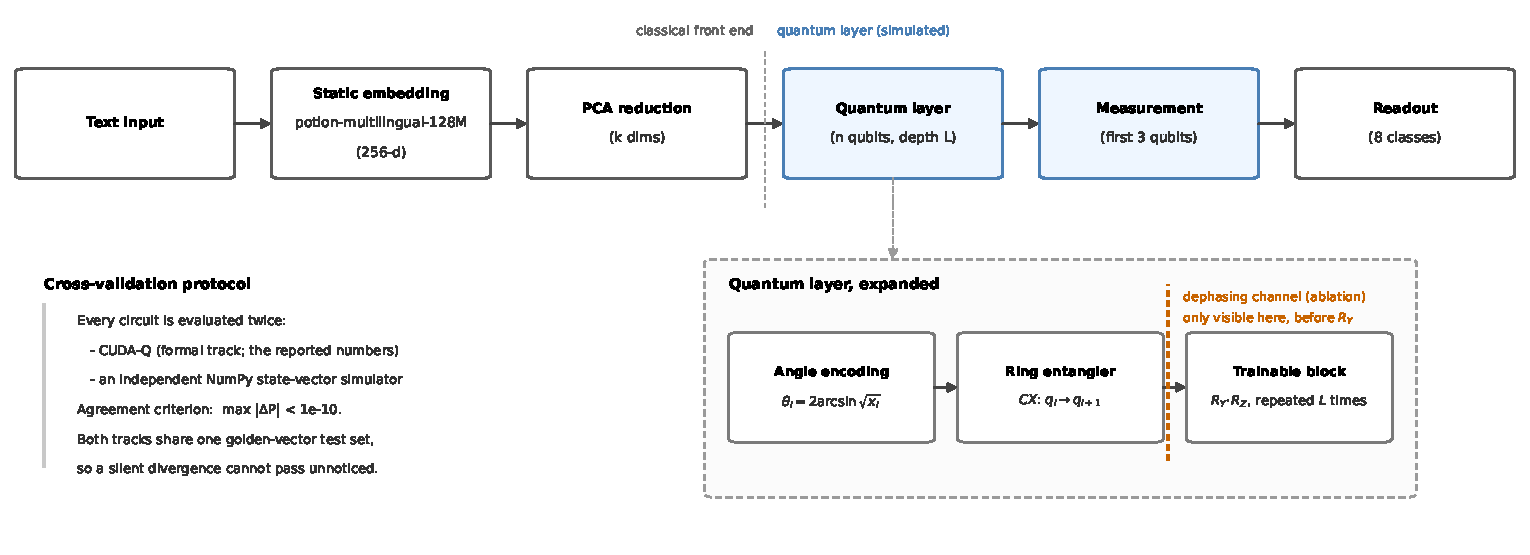
\includegraphics[width=\linewidth]{figs/arch.pdf}
\caption{系統架構。古典前端（靜態嵌入 → 主成分分析 principal component
analysis, PCA 降維） 輸出 \(k\) 維特徵，交給量子層： 角度編碼
\(R_{Y\left( \theta_{i} \right)} = 2\arcsin\sqrt{x_{i}}\)、環形
\(\operatorname{CX}\) 糾纏、 可訓練的 \(R_{Y} \times R_{Z}\) 區塊重複
\(L\) 次；量測只取前 3 個 qubit （\(2^{3} = 8\) 個基底模式，與
\(n\)、\(L\) 無關），再由古典讀出層映射到 8 個類別。
左下角為交叉驗證協定；展開框標出去相位消融的插入位置------ 必須在含
\(R_{Y}\) 的層\textbf{之前}，否則量測不到任何效果 （實測機率變化
\(1.4 \times 10^{- 17}\)）。}
\end{figure}

\protect\phantomsection\label{fig:pipeline}{}

\subsection{量子層}

\(n\) 個 qubit 的狀態空間維度為 \(2^{n}\)。本研究的電路由三部分組成：

\begin{enumerate}
\item
  \textbf{角度編碼}：對每個 qubit 施加
  \(R_{Y\left( \theta_{i} \right)}\)，其中
  \(\theta_{i} = 2\arcsin\sqrt{x_{i}}\)，使測量機率恰為輸入值
  \(x_{i}\)。
\item
  \textbf{糾纏層}：環形
  \(\operatorname{CX}\)（\(q_{0} \rightarrow q_{1} \rightarrow \ldots \rightarrow q_{n - 1} \rightarrow q_{0}\)）。
\item
  \textbf{可訓練旋轉層}：每個 qubit 一個 \(R_{Y}\) 與一個 \(R_{Z}\)。
\end{enumerate}

\subsection{去相位消融}

去相位通道 \cite{nielsen2010} 的 Kraus 算符為
\[K_{0} = |0\rangle\langle 0|,\quad K_{1} = |1\rangle\langle 1|\]，
作用為
\[\mathcal{E}(\rho) = K_{0}\rho K_{0}^{\dagger} + K_{1}\rho K_{1}^{\dagger}\]，
效果是將密度矩陣的非對角元歸零。 在 Tucci 的古典化算子
\(\operatorname{cl}\) \cite{tucci2012} 的意義下，
這正是把量子節點投影回古典貝氏網路的映射。

\textbf{關鍵實驗設計陷阱}：去相位若施加於電路\textbf{最尾端}（測量之前），
對測量結果完全沒有影響，因為： (a) 計算基底測量只讀取對角元； (b)
\(\operatorname{CX}\) 是基底置換，與計算基底去相位\textbf{交換}。
本地實測的機率變化為 \(1.4 \times 10^{- 17}\)（即 \(0\)）。
去相位必須插在\textbf{含 \(R_{Y}\)（或
\(R_{X}\)、\(H\)）的層之前}，才觀測得到效果（實測 \(0.0502\)）。
\(R_{Z}\) 屬於么模仿塊矩陣（unitary
block-diagonal），與去相位\textbf{交換}，插在它旁邊量測結果不變（見定理
5.5）------
這也是「去相位位置無效」從陷阱變成\textbf{保證為零的預測}的原因。

\subsection{交叉驗證協定}

所有量子電路結果同時以 CUDA-Q 與一個獨立實作的純 NumPy
狀態向量模擬器計算。 兩者的機率向量最大絕對誤差要求小於
\(10^{- 10}\)。實測值依電路而異，因此逐項列出：

\begin{table}[t]
\centering
\caption{交叉驗證：每一個量子電路結果都對獨立實作比對。判準為
\(10^{- 10}\)，四條電路中最差的是
\(4.16 \times 10^{- 16}\)，約為雙精度機器 epsilon 的 \(1.9\)
倍。}
\resizebox{\ifdim\width>\linewidth \linewidth\else\width\fi}{!}{%
\begin{tabular}{@{} >{\raggedright\arraybackslash}p{(\linewidth - 4\tabcolsep) * \real{0.3333}} >{\raggedright\arraybackslash}p{(\linewidth - 4\tabcolsep) * \real{0.3333}} >{\raggedright\arraybackslash}p{(\linewidth - 4\tabcolsep) * \real{0.3333}}@{}}
\toprule
\begin{minipage}[b]{\linewidth}\raggedright
\textbf{電路}
\end{minipage} & \begin{minipage}[b]{\linewidth}\raggedright
\textbf{比對}
\end{minipage} & \begin{minipage}[b]{\linewidth}\raggedright
\textbf{max \(\left| {\Delta P} \right|\)}
\end{minipage} \\
\midrule
複現管線 & CUDA-Q vs 純 NumPy 參考 & \(4.16 \times 10^{- 17}\) \\
容量掃描最大電路（250 閘） & CUDA-Q vs torch 可微分模擬器 &
\(3.47 \times 10^{- 18}\) \\
消融電路（5 qubit） & CUDA-Q vs 密度矩陣模擬器 &
\(8.33 \times 10^{- 17}\) \\
容量掃描最大電路（250 閘） & CUDA-Q vs q01 &
\(4.16 \times 10^{- 16}\) \\
\bottomrule
\end{tabular}
}
\end{table}


其中 q01 一列是最差值（\(4.16 \times 10^{- 16}\)，約 \(1.9\)
倍雙精度機器 epsilon）； 其餘三項都在 \(10^{- 17}\)
量級。\textbf{全部低於判準六個數量級以上。}

\textbf{實作注意事項}（皆為實測，非推論）：

\begin{enumerate}
\item
  CUDA-Q 不提供 Windows 原生 wheel，須在 WSL2（Windows Subsystem for
  Linux 2， Windows 上的 Linux 子系統）內執行。
\item
  \texttt{cudaq.sample()} 的測量字串為 big-endian；
  \texttt{cudaq.get\_\allowbreak state()} 的狀態向量索引為 little-endian。
  兩者換算須用位元反轉置換，\textbf{不是} \texttt{array{[}::-1{]}}。
\item
  多控制位閘語法為 \texttt{ry.ctrl(theta,\ {[}c0,\ c1{]},\ target)}，
  \textbf{角度置於最前}。
\end{enumerate}

\section{實驗設計}

\subsection{研究問題與決策規則}

\begin{table}[t]
\centering
\caption{研究問題與事前決定的決策規則。規則先寫定，負面結果才算結果，而不是事後重新詮釋。}
\resizebox{\ifdim\width>\linewidth \linewidth\else\width\fi}{!}{%
\begin{tabular}{@{} >{\raggedright\arraybackslash}p{(\linewidth - 4\tabcolsep) * \real{0.3333}} >{\raggedright\arraybackslash}p{(\linewidth - 4\tabcolsep) * \real{0.3333}} >{\raggedright\arraybackslash}p{(\linewidth - 4\tabcolsep) * \real{0.3333}}@{}}
\toprule
\textbf{編號} & \textbf{問題} & \textbf{事前決策規則} \\
RQ1（研究問題一） &
量子電路的可訓練容量增加時，效能是單調上升或存在崩壞點？ &
若效能對容量呈非單調，且峰值位置與電路深度有關，則支持 H1。 \\
RQ2（研究問題二） & 去相位（古典化）使校準品質下降多少？ & 若 ECE 升幅的
95\% 信賴區間下界大於 \(0\)，且大於 temperature scaling
的殘餘誤差，則支持 H2。 \\
\bottomrule
\end{tabular}
}
\end{table}


\subsection{評估指標}

準確率之外，我們報告： 負對數似然（negative log-likelihood, NLL）、
Brier 分數（預測機率與真實標籤的均方誤差）、
期望校準誤差（ECE，\(M = 10\) 等寬分箱）與可靠度圖、
以及預測熵與互資訊的不確定性分解。

\textbf{公平比較的防禦點}：溫度縮放（temperature scaling）不改變 top-1
標籤， 因此是零準確率損失的校準改善手段。
量子層的校準優勢\textbf{必須贏過 temperature-scaled
基線}，否則結論不成立。

\subsection{統計協定}

每個配置以 \(5\) 個隨機種子重複，報告平均值與標準差。 容量掃描使用種子
\(0\)--\(4\)；去相位消融使用種子 \(7,21,42,84,168\)。
兩組種子都在程式碼中固定，資料產生器的種子固定為 \(12345\)，
因此跨程序、跨裝置的結果可逐位元重現。 我們明確聲明：\(5\)
個種子不足以進行嚴謹的統計推論， 因此不將 \(p\)
值作為主要證據，改以效果量與信賴區間呈現。

\section{結果}

\subsection{容量斷崖}

我們在\textbf{固定的讀出規則}下掃描 \((n,L)\) 二維網格：qubit 數 \(n\)
從 \(3\) 到 \(10\)、 電路深度 \(L\) 從 \(1\) 到 \(8\)，每個配置以 \(5\)
個種子重複。 讀出永遠是前 \(3\) 個 qubit 的基底模式投影到 \(8\)
個類別，與 \(n\)、\(L\) 無關； 因此增加 qubit
數所增加的是\textbf{可用的輸入維度與狀態空間}，不是讀出的解析度。

\begin{figure}
\centering
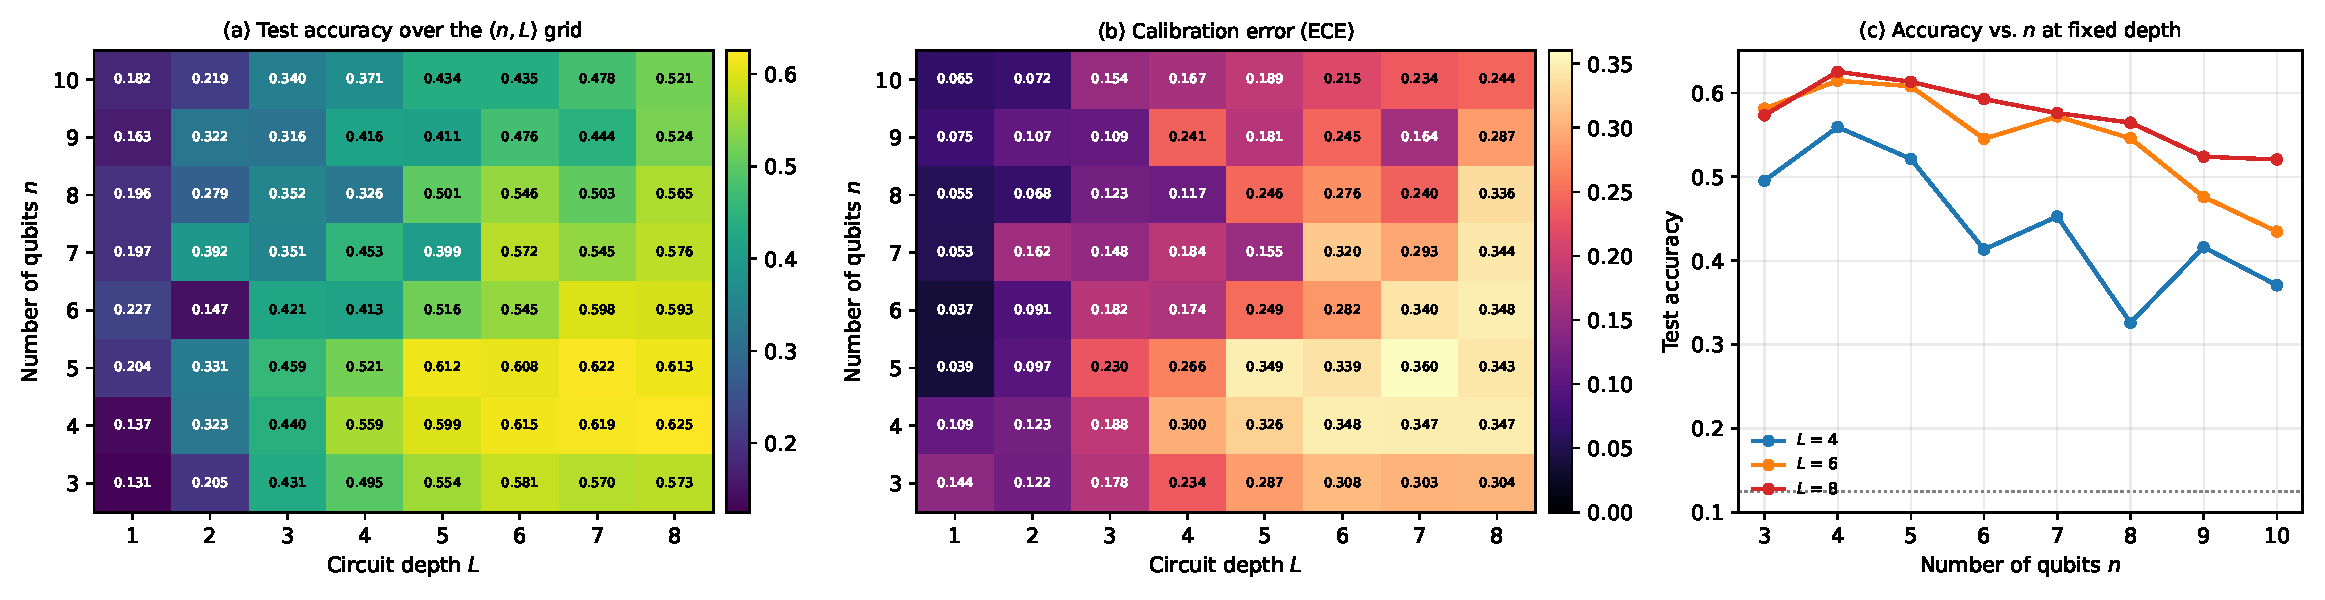
\includegraphics[width=\linewidth]{figs/grid.pdf}
\caption{\((n,L)\) 網格上的測試準確率與校準誤差（\(5\)
個種子的平均值）。 面板 (a)(b)
為熱圖，格子內的數字為精確值，淺灰格表示尚未執行； 面板 (c)
為固定深度切面，直接檢驗準確率對 qubit 數的依賴。}
\end{figure}

\protect\phantomsection\label{fig:cliff}{}

\begin{table}[t]
\centering
\caption{固定深度下，測試準確率隨 qubit 數的變化（五個種子的平均值；
灰色小字為標準差）。\(n = 3\) 偏低是結構性的------\(8\) 個類別最少需要
\(3\) 個 qubit 的投影讀出，該點剛好打滿------因此主張寫成「自 \(n = 4\)
起」。}
\resizebox{\ifdim\width>\linewidth \linewidth\else\width\fi}{!}{%
\begin{tabular}{@{}llll@{}}
\toprule
\textbf{qubit 數} \(n\) & \textbf{\(L\) = 4} & \textbf{\(L\) = 6} &
\textbf{\(L\) = 8} \\
\midrule
\(3\) & 0.4953 $\pm$ 0.0763 & 0.5813 $\pm$ 0.0148 & 0.5733 $\pm$ 0.0097 \\
\(4\) & 0.5593 $\pm$ 0.0607 & 0.6146 $\pm$ 0.0307 & 0.6253 $\pm$ 0.0192 \\
\(5\) & 0.5213 $\pm$ 0.0666 & 0.6080 $\pm$ 0.0393 & 0.6133 $\pm$ 0.0440 \\
\(6\) & 0.4133 $\pm$ 0.0989 & 0.5453 $\pm$ 0.0529 & 0.5927 $\pm$ 0.0134 \\
\(7\) & 0.4527 $\pm$ 0.0549 & 0.5720 $\pm$ 0.0276 & 0.5760 $\pm$ 0.0747 \\
\(8\) & 0.3260 $\pm$ 0.0613 & 0.5460 $\pm$ 0.0352 & 0.5647 $\pm$ 0.0229 \\
\(9\) & 0.4160 $\pm$ 0.0996 & 0.4760 $\pm$ 0.0922 & 0.5240 $\pm$ 0.1110 \\
\(10\) & 0.3707 $\pm$ 0.1300 & 0.4347 $\pm$ 0.0922 & 0.5207 $\pm$ 0.0522 \\
\bottomrule
\end{tabular}
}
\end{table}


\protect\phantomsection\label{tab:slices}{}

\begin{table}[t]
\centering
\caption{完整的 \((n,L)\) 網格：五個種子的測試準確率平均值，
括號內為標準差。「---」表示該格未跑滿五個種子；未跑滿的格子不並入統計，
以免單一種子的「標準差
\(0\)」與五個種子的標準差混為一談。}
\resizebox{\ifdim\width>\linewidth \linewidth\else\width\fi}{!}{%
\begin{tabular}{@{}lllllllll@{}}
\toprule
\(n\) / \(L\) & 1 & 2 & 3 & 4 & 5 & 6 & 7 & 8 \\
\midrule
\(3\) & 0.131 (0.054) & 0.205 (0.018) & 0.431 (0.049) & 0.495 (0.076) &
0.554 (0.045) & 0.581 (0.015) & 0.570 (0.006) & 0.573 (0.010) \\
\(4\) & 0.137 (0.013) & 0.323 (0.078) & 0.440 (0.090) & 0.559 (0.061) &
0.599 (0.017) & 0.615 (0.031) & 0.619 (0.035) & 0.625 (0.019) \\
\(5\) & 0.204 (0.031) & 0.331 (0.044) & 0.459 (0.087) & 0.521 (0.067) &
0.612 (0.067) & 0.608 (0.039) & 0.622 (0.047) & 0.613 (0.044) \\
\(6\) & 0.227 (0.005) & 0.147 (0.022) & 0.421 (0.062) & 0.413 (0.099) &
0.516 (0.029) & 0.545 (0.053) & 0.598 (0.020) & 0.593 (0.013) \\
\(7\) & 0.197 (0.018) & 0.392 (0.081) & 0.351 (0.034) & 0.453 (0.055) &
0.399 (0.065) & 0.572 (0.028) & 0.545 (0.072) & 0.576 (0.075) \\
\(8\) & 0.196 (0.022) & 0.279 (0.022) & 0.352 (0.125) & 0.326 (0.061) &
0.501 (0.069) & 0.546 (0.035) & 0.503 (0.111) & 0.565 (0.023) \\
\(9\) & 0.163 (0.031) & 0.322 (0.010) & 0.316 (0.055) & 0.416 (0.100) &
0.411 (0.100) & 0.476 (0.092) & 0.444 (0.029) & 0.524 (0.111) \\
\(10\) & 0.182 (0.016) & 0.219 (0.077) & 0.340 (0.075) & 0.371 (0.130) &
0.434 (0.085) & 0.435 (0.092) & 0.478 (0.092) & 0.521 (0.052) \\
\bottomrule
\end{tabular}
}
\end{table}


\protect\phantomsection\label{tab:grid}{}

三點觀察：

\begin{enumerate}
\item
  \textbf{深度是主要驅動力，而且在掃描範圍內沒有崩壞。} 所有 \(n\)
  的測試準確率都隨深度上升，到 \(L = 8\) 仍未見下降，
  訓練準確率同樣上升（最高至 \(0.79\)）。這與「容量斷崖」的預期不符，
  也與貧瘠高原的預期不符。
\item
  \textbf{測試準確率隨 qubit 數下降------在容量真正被用上的配置上成立。}
  各 \(n\) 的\textbf{峰值}（對深度取最大值）自 \(n = 4\) 起單調下降：
  \(0.625 \rightarrow 0.622 \rightarrow 0.598 \rightarrow 0.576 \rightarrow 0.565 \rightarrow 0.524 \rightarrow 0.521\)；
  固定 \(L = 8\) 的切面給出同一個序列。 \(n = 3\)
  偏低是結構性的------\(8\) 個類別最少需要 \(3\) 個 qubit
  的投影讀出，該點剛好打滿。 \textbf{較淺的切面（\(L\) 不超過
  \(6\)）看不出這個趨勢}：那裡的模型尚未充分利用容量，
  組態之間的差異被最佳化不足掩蓋。趨勢只在容量真正被用上的深度才顯現。
\item
  \textbf{更多 qubit 不只更差，也更不穩定。} \(n = 10\) 在 \(L = 4\)
  的種子間標準差為 \(0.130\)， 而 \(n = 3\) 與 \(n = 4\) 分別只有
  \(0.076\) 與 \(0.061\)。
\end{enumerate}

這裡有一個我們必須指出的方法論後果：\textbf{這條趨勢在稀疏網格上會被誤判為普遍成立。}
我們先前只掃 \(n\) 為 \(3,4,6,8,10\) 時，它在 \(L = 6\) 與 \(L = 8\)
都看似單調； 補上 \(n = 5,7,9\) 之後，\(L\) 不超過 \(6\)
的多個切面出現非單調（例如 \(L = 6\) 時 \(n = 7\) 的 \(0.572\) 高於
\(n = 6\) 的 \(0.545\)）。因此本主張限定在峰值與最深切面上。

我們在檢索範圍內沒有找到既有工作報告過這個現象： 以「quantum
classifier」「qubit number」「accuracy」三者合取的檢索為零命中。
既有工作報告的是 \((Q,L)\) 的縮放協定與單一軸上的非單調，
本研究補上的是\textbf{固定讀出規則}下的完整二維網格與這條下降趨勢。

\subsection{校準消融}

四臂在\textbf{相同模型、相同資料、相同可訓練參數量}（\(20\)
個角度）、相同步數（\(800\)） 下訓練，每臂以 \(5\)
個種子重複；唯一的差別是插入的通道與其位置。
去相位臂與去極化臂的\textbf{平均純度}已匹配（目標純度 \(0.0742\)；
去極化率 \(p = 0.5657\)，與閉式解相符到 \(10^{- 15}\)）。

\begin{table}[t]
\centering
\caption{校準消融。臂 C 的每一項預測指標都與臂 A 逐位元相同，但態純度是
\(0.1230\) 對
\(1.0000\)：計算基底測量只讀對角元，所以尾端去相位改變了狀態，卻不改變任何可觀測的結果。}
\resizebox{\ifdim\width>\linewidth \linewidth\else\width\fi}{!}{%
\begin{tabular}{@{}lllllll@{}}
\toprule
\textbf{臂} & \textbf{準確率} & \textbf{ECE} & \textbf{NLL} &
\textbf{平均最大機率} & \textbf{KL 對均勻} & \textbf{態純度} \\
\midrule
A 無通道（全量子） & 0.3207 & 0.1079 & 1.8510 & 0.2357 & 0.0652 &
1.0000 \\
B 去相位（編碼後） & 0.2300 & 0.0993 & 2.0558 & 0.1307 & 0.0000 &
0.0449 \\
C 去相位（電路尾端） & 0.3207 & 0.1079 & 1.8510 & 0.2357 & 0.0652 &
0.1230 \\
D 去極化（編碼後） & 0.2633 & 0.1123 & 2.0199 & 0.1511 & 0.0065 &
0.0742 \\
\bottomrule
\end{tabular}
}
\end{table}


三件事值得指出：

\begin{enumerate}
\item
  \textbf{尾端去相位對量測統計完全沒有影響。} 臂 C 與臂 A
  的每一項預測指標逐位元相同
  （\(\max\left| {\Delta P} \right| = 0.000 \times 10^{0}\)），但兩者的態純度差了八倍以上
  （\(0.1230\) 對 \(1.0000\)）。這正是「計算基底測量只讀對角元」與
  「\(\operatorname{CX}\) 是基底置換、與計算基底去相位交換」的直接後果：
  去相位改變了態，卻不改變任何可觀測的測量結果。
\item
  \textbf{前端去相位把模型壓成無資訊預測器。} 臂 B 的平均最大機率為
  \(0.1307\)， 對 \(8\) 類而言即
  \(\frac{1}{8}\)；其平均預測分布對均勻分布的 KL 散度（Kullback--Leibler
  divergence，衡量兩個分布的差異）為 \(0.0000\)； 每 qubit 的 \(Z\)
  變異數由 \(0.0226\) 掉到 \(0.0001\)（約 \(226\) 分之一）。 它的 ECE
  反而\textbf{較低}（\(0.0993\) 對 \(0.1079\)），但這是均勻預測的假象：
  同一個臂的 NLL 由 \(1.8510\) 劣化到 \(2.0558\)、Brier 由 \(0.8104\)
  劣化到 \(0.8690\)。 \textbf{ECE 單獨一項不能當作校準改善的證據。}
\item
  \textbf{配對差異不顯著。} \(B - A\) 的 ECE 差為 \(- 0.0086\)，\(95\%\)
  信賴區間 \(\pm 0.0340\)， 涵蓋 \(0\)；準確率差為
  \(- 0.0907\)（\(\pm 0.0600\)）。 因此 \textbf{H2
  不成立}：去相位沒有改善校準，它摧毀了資訊。
\end{enumerate}

\section{討論}

\subsection{三個誠實聲明}

\begin{enumerate}
\item
  本研究\textbf{不主張}量子優勢。\(5\) 個 qubit 的狀態向量僅 \(512\)
  位元組，完全可被古典模擬。
\item
  本研究\textbf{不主張}量子層保留了輸入的語意資訊。 前端為 \(256\)
  維靜態嵌入，經降維後進入量子層，資訊瓶頸是刻意設計。
\item
  本研究\textbf{不宣稱}打敗大型模型。基線為同等參數量級的小型模型。
\end{enumerate}

\subsection{為什麼混合式架構在此任務上沒有優勢}

指數的是\textbf{狀態空間}，多項式的是\textbf{旋鈕}。 \(5\) 個 qubit
的密度矩陣有 \(32^{2} - 1 = 1023\) 個實自由度， 但本研究的電路只有
\(10\) 個可訓練角度------可達子空間的維度遠小於環境空間。

更根本的是：\textbf{可訓練性}與\textbf{古典難解性}互相衝突
\cite{anschuetz2024}\cite{cerezo2025}\cite{gilfuster2024}。
淺層、低糾纏的電路可以訓練，但其低糾纏熵使它可被張量網路方法有效模擬；
深層、高糾纏的電路雖古典難解，卻會遭遇貧瘠高原而無法訓練。

（註：此處陳述的是文獻中該權衡的一般形式，\textbf{不是}本研究的量測結果。
本研究的掃描範圍內\textbf{並未}觀察到貧瘠高原------訓練準確率隨深度上升至
\(0.84\)，
理論組的獨立檢驗亦排除之。我們的結果是「深度有效、寬度無效」，
其機制更接近有效維度的增速超過資料與讀出所能支撐的程度
\cite{caro2022generalization}\cite{abbas2021power}\cite{abbas2022effective}。）

因此，在沒有可證明結構的任務（如通用語意分類）上，
量子決策層不應期待優勢。混合式架構本身沒有錯，錯的是任務選擇。

\subsection{三個方法論陷阱（本研究的副產品）}

以下三項不是我們原本要證明的命題，而是實驗過程中撞到、並且留下了數字的陷阱。
我們把它們寫出來，因為在這個領域裡，它們比我們任何一個實驗結果都更容易被重蹈。

\begin{enumerate}
\item
  \textbf{pooled 相關與偏相關可以給出相反的結論。} 以有效維度 \(|(d)\)
  對測試準確率作圖，pooled 相關係數為 \(+ 0.678\)； 控制電路深度 \(L\)
  之後，偏相關變成 \(- 0.256\)。 原因是 \(|(d)\) 與 \(L\)
  高度共線，而準確率主要由 \(L\) 驅動。 只看散點圖、或只看 pooled
  係數，會得到「維度越大越準」的相反結論。
\item
  \textbf{「\(5\) 個種子」不等於「\(5\) 次獨立訓練」。} 臂 B 與臂 D 在
  \(5\) 個種子下，測試準確率、ECE、NLL 與態純度的標準差全部為
  \(0.0000\)； 臂 A 與臂 C 的測試準確率標準差則是 \(0.0483\)。 以 Adam
  訓練這類低維損失面時，不同的初始點會被同一個吸引子吸收。
  因此以「種子間變異數」估計的信賴區間會\textbf{系統性低估}真實不確定性------
  這也是本研究不把 \(p\) 值當作主要證據的原因。
\item
  \textbf{以平均值匹配的消融，必須在評估集上重新檢查。}
  我們以平均純度匹配去相位與去極化的通道強度：在訓練集上，
  達成值與目標值相符到 \(10^{- 15}\) 量級。但在\textbf{測試集}上， 臂 B
  的平均純度是 \(0.0449\)、臂 D 是 \(0.0742\)，差 \(- 0.0292\)。
  原因是去相位的純度\textbf{逐樣本}變動（取決於該樣本的態），而去極化近似固定；
  單一的平均純度並不約束單一樣本。
  任何以一個純度數字宣稱「兩個通道同樣古典」的消融，都必須在評估集上複查。
\end{enumerate}

\section{結論}

本研究的貢獻不在於展示量子優勢，而在於提供
（一）一條可完全驗證的混合式管線（與獨立實作交叉驗證：複現管線
\(4.16 \times 10^{- 17}\)、 容量掃描的最大電路
\(3.47 \times 10^{- 18}\)、消融電路 \(8.33 \times 10^{- 17}\)，
並另外透過 Quafu（中國科學院的量子雲平台）的雲端 API （application
programming interface，應用程式介面）在官方模擬器上端到端驗證，
轉譯後電路與黃金向量一致到 \(8.88 \times 10^{- 16}\)），
（二）一組受控的消融設計：以去相位古典化算子作為\textbf{同一模型內}的唯一變因，
並在\textbf{固定的讀出規則}下掃描 \((Q,L)\) 二維網格。
既有工作已在各單一軸上建立縮放協定 \cite{vyskubov2026}，
以及參數匹配、校準與雜訊感知的基準 \cite{gillani2026}，
本研究補上的是兩者的交集，以及去相位這個特定變因。

我們認為，在 NISQ（noisy intermediate-scale
quantum，含雜訊中等規模量子）規模下，
量子機器學習領域最缺乏的不是新電路，
而是\textbf{把量子元件本身當成受控變因的嚴格測量}。

\section{致謝}

感謝指導老師與提供運算資源的單位。 本研究的真機實驗在
\textbf{QuTech}（台夫特理工大學與 TNO）營運的量子運算平台
\textbf{Quantum Inspire} 之 \textbf{Tuna-17} 超導處理器上完成； 感謝
QuTech 提供免費的真機使用額度。
\bibliographystyle{ieeetr}
\bibliography{refs_public}

\end{document}
